\documentclass[dvipdfmx]{jsarticle}
\usepackage[dvipdfmx]{graphicx}

\title{コミュニケーション論:時間割外演習}
\author{澤 \/ 祐里(21--1--037--0801)}
\date{\today} 

\begin{document}
\maketitle

\section{課題の目的}

技術の進歩により、様々なコミュニケーションの壁が克服されてきた。
しかしながら、現代においても様々なコミュニケーションの問題、たとえ
ば伝達意図が誤解される、意図が伝わらない、といった事例が少なか
らず起きている。このような伝達意図が正しく伝わらない状況がなぜ起
きるのか、これまでの授業内容をもとに自分なりに考察せよ。
また、よりよいコミュニケーションのために、情報技術に何が出来るか、
自分なりの意見を述べよ。その際、そのように考えた判断の根拠を示し
ながら論ぜよ。

\section{考察}
\begin{itemize}
  \item コミュニケーションとは、人々の間で、知識、アイデア、考え、概念や感情のやり取りをすることである。
  話し手は自身の思い描くものを相手に伝えるために、言語や仕草などの「話し手と聞き手で共通の意味を持ったコード」に変換して
  、聞き手に伝える。それに対して、聞き手は、受け取ったコードを解読して、伝達内容を再構成する。
  他にも、「コンテクスト依存コミュニケーション」と呼ばれるコミュニケーションでは、聞き手が文脈(コンテクスト)を参照しながら
  、話してが想定したであろうコードを逆算的に推定する。このコミュニケーションでは、聞き手は主体的に推論を行う営み、すなわち
  解釈を行う。
  \begin{itemize}
    \item[→] コミュニケーションの問題は、上記のコミュニケーションを行う際に、
    話し手のメッセージに盛り込んだ情報が、聞き手に過不足なく伝わらなかった際に起こってしまう。
    以下に、話し手のメッセージが聞き手に過不足なく伝わらない原因として考えられるものを列挙する。
    \begin{itemize}
      \item 話し手と聞き手に知識差などが存在し、互いのコードに差異が存在する。
      \\例えば、日本人が外国人に対して、話しかけたとしても上手くコミュニケーションをとることはできない。なぜなら、
      外国人は日本語を知らないため、日本人が話している内容を理解することができないためである。
      これは外国人だけでなく、同じ日本人であったとしても、話し手が使っている日本語の意味と
      聞き手が知っているその日本語の意味に間違いがあったり、聞き手がその日本語の意味を知らない可能性もある。
      例えば、「今度はエラーが出なかったので、出来たと思ったら、前と同じ結果だった。アプリケーションサーバを再起動して
      いなかったので、前のが動いていただけだった。」というような文は、日本語である。
      しかし、この分を理解するためには、日本語だけではなく、プログラムの知識や作業の流れ、それぞれの作業の関連性などの
      構造化された知識が必要となる。そのため、このような知識を共有出来ていない相手とは、互いのコードに差異が生じてしまう。
      また、「右の方を3の5でお願いします」のような文は、ひとつひとつの言葉の意味は理解することができ、文法的にも間違ってはいない。
      しかし、これだけでは、意味を理解することはできない。だが、この文が機械の操作パネルの前で行われた会話であるならば、
      「(操作パネルの)右のほうを3(つめのスイッチ)の(値を)5でお願いします」というような解釈をすることができる。
      これは、コミュニケーションをとった時の環境情報や会話の前後の文脈、他者の存在、社会的な文脈などから意味を判断しており、
      これらの手掛かりを相手と自分の間で共有しているからこそ意味が伝わる。
      そのため、これらの手掛かりを共有出来ていない場合などは、互いのコードに差異が生じてしまう。
      \item 聞き手が自らの主体的解釈を通じて、発信者の意図を超えたメッセージに読み取ってしまう。
      \\1999年に起きたJCO東海事業所の臨界事故では、核燃料加工施設内で核燃料を加工していた最中、ウラン溶液が臨界に達して
      核分裂連鎖反応が発生し、至近距離で中性子線を浴びた作業員3名中、
      2名が死亡、1名が重症となったほか、667名の被曝者を出した。
      この事故は、JCOのずさんな作業工程管理が原因ではあるものの、作業員にはマニュアルはきちんと配られていた。
      それにも関わらず、この大事故が起こってしまったのは、マニュアルの重要性が伝わっていなかったからであると考えられる。
      これは、聞き手である作業員達の主体的解釈を通じて、マニュアルの重要性を見誤ってしまい、
      面倒な作業は省く程度の感覚で作業を行ってしまったと考えられ、その結果として大事故が起こってしまった。
      \item 言語理解のためには、言語メッセージ以外の情報も必要となる。
      \\会話はその場にふさわしいように、話者、聞き手はお互いに共同しあう(協調の原則)ことが前提の場合。
      例えば、「カラオケに行かない?」という問いに対して、「明日、テストがあるんだ」という返答は字義通りに
      解釈すると返答になっていない。しかし、聞き手は、話者が間違ったことを言ったり、誤解を与えようとしているわけではなく、
      別の意味があるはずだと解釈をする。そのため、「明日、テストがあるから、カラオケには行けない」という風に解釈を
      することができる。他にも、「お腹すいたなあ」ということに対して、「まっすぐ行くと焼きマンがあるよ」という返答は、
      お腹がすいたということに対して、「焼きマン」なるものの道案内をしている。ここから、聞き手は、「焼きマン」なるものが
      食事をする場所であるという含意を知る。
      このように、会話の含意を理解するには、聞き手が協調の原則や、会話の公理を理解しているだけでなく、解釈
      のための背景知識(文脈や状況)が必要となる。また、人間の対面型コミュニケーションでは、
      言語情報、表情、声のトーンなどの要素があり、これらの要素が互いに矛盾なメッセージを
      送った場合、どの要素からの情報を重要視するかという実験では、
      言語情報が7%、言語以外の聴覚情報が38%、視覚情報が55%となっており、非言語の要素が93%も占めている
      (Mehrabianの法則)。この法則は、好き嫌いなどの感じ方や態度に関すること以外には適用できないが、
      言語メッセージ以外の情報も重要であることが分かる。
      これらのことを考えると、言語メッセージのみを真に受けてしまうのは、解釈にズレが生じてしまう原因となる。
    \end{itemize}
    上記のことを考えると、コミュニケーションは、「自分が話したいこと」を相手に伝えるだけでは上手くいかないことが分かる。
    そのため、コミュニケーションは相手の知識や興味を考えて話さなければ成り立たず、
    人によって知識や興味は変わることから、相手によって話し方や話す内容は変えなければいけないことが分かる。
    そして、相手によって話す内容を変える必要があることから、「どう伝えるか」などよりも、
    伝える内容が重要となることが分かる。
  \end{itemize}
\end{itemize}
\begin{itemize}
  \item よりよいコミュニケーションのために、情報技術に何が出来るか
  \begin{itemize}
    \item[→] 私たち人間のコミュニケーションでは、言語だけでも、文脈や状況などで意味が違ったり、
    文を正しく解釈するために背景知識が必要だったりと、文一つがとても複雑で、
    AIに理解させることは、非常に難しいと考えられる。
    しかし、そのような難しいコミュニケーションを情報技術のおかげで、
    人間はより簡単にコミュニケーションをとれるようになった。
    例えば、
    webや動画サイトなどのような技術では、様々な情報に簡単にアクセスすることができ、
    また、メールやzoomなどのように、任意の相手と簡単にコミュニケーションをとることができる。
    よりよいコミュニケーションを行うために重要な伝える内容を人間に与えていることから、
    webや動画サイトは人間がコミュニケーションをとる際の手助けとなっていることが分かる。
    また、情報検索機能の発展により、必要な情報を迅速に入手することができ、
    自然言語処理を用いた情報技術により、カテゴリ別のトレンドなどを把握することができる。
    メールやzoomでは、実際に対面で話しているわけではないため、自分の意見を
    比較的言いやすくなり、課題志向的になる。また、端末とネット環境さえあれば、どこからでも
    コミュニケーションをとることができるため、人間のコミュニケーションの難易度を下げていることが
    分かる。特にzoomでは、カメラを通して相手の表情を見たり、
    画面の共有などで視覚情報も共有することができるため、
    通話よりも深くコミュニケーションをとることができる。
    twitterやfacebookなどといったsnsでは、個人が情報を発信する場を提供しており、
    さらに、人と人がインターネット上でコミュニケーションをとる場を提供している。
    他にも、Google翻訳などの翻訳機能は、他言語を扱う人々ともコミュニケーションを
    可能にすることができるものであり、他言語で書かれた最新の研究や書物などにもアクセスすることが
    できるため、得られる情報の幅も広がる。
    このように、情報技術は、人とコミュニケーションをとるための話の内容の提供から、個人が情報を発信する場の提供
    も行っており、さらには、様々な人々と容易にコミュニケーションをとる手段の提供も行っている。
    これらのことから、情報技術のおかげで、人間はコミュニケーションを取りやすいようになっており、
    今後の情報技術の発展においても、同様に人間のコミュニケーションをより手助けできるように
    なることが考えられる。特に近年では、ディープラーニングが発展しており、
    その影響で自然言語処理の分野も発展している。
    例えば、図\ref{graph:1}のような、AIによる「自動要約」の技術は、ニュースなどの重要な部分などを抜き出して
    見ることができ、短時間で1日の話題を作ることができる。
  \end{itemize}
\end{itemize}
\begin{figure}[b]
  \centering
  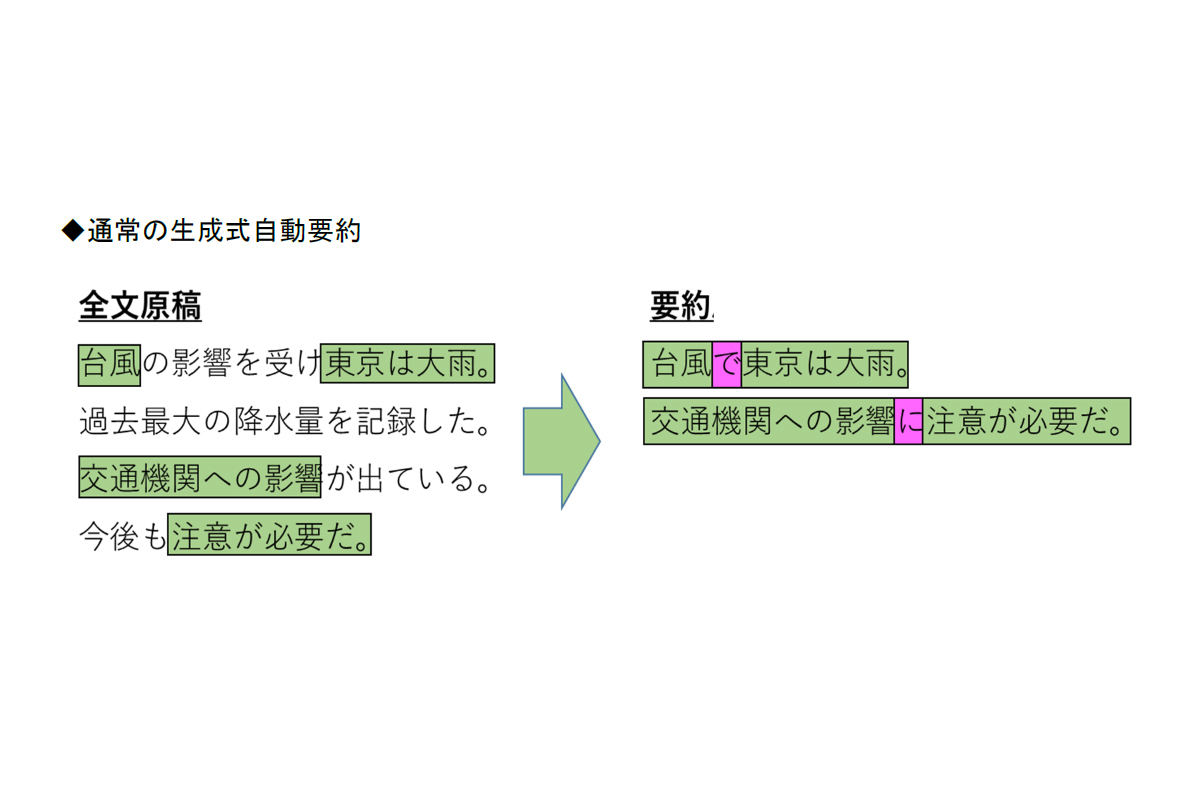
\includegraphics[keepaspectratio, scale=0.19]{003.jpg}
  \caption{自動要約}
  \label{graph:1}
\end{figure}

\end{document}